\documentclass{beamer}

\usepackage[utf8]{inputenc}
\usepackage[T1]{fontenc}
\usepackage{lmodern}
\usepackage[french]{babel}

% \usepackage[usenames,dvipsnames,svgnames,table]{xcolor}

\usepackage{amsmath}
\usepackage{amssymb}
% \usepackage{mathrsfs}

\usepackage{scrextend}

\usepackage{listings}
\definecolor{listinggray}{gray}{0.9}
\definecolor{lbcolor}{rgb}{0.95,0.95,0.95}
\lstset{
	backgroundcolor=\color{lbcolor},
	tabsize=4,
	rulecolor=,
	language=Java,
	basicstyle=\small\ttfamily,
	upquote=false,
	aboveskip={.5\baselineskip},
	columns=fixed,
	showstringspaces=false,
	extendedchars=true,
	showspaces=false,
	breaklines=true,
	prebreak = \raisebox{0ex}[0ex][0ex]{\ensuremath{\hookleftarrow}},
	frame=single,
	showtabs=false,
	identifierstyle=\ttfamily,
	keywordstyle=\bfseries\color[rgb]{0,0,1},
	commentstyle=\color[rgb]{0.133,0.545,0.133},
	stringstyle=\color[rgb]{0.627,0.126,0.941},
}


% --------------------
% Configuration Beamer
% --------------------

\usetheme{Warsaw}
% Pour troller en copiant Jube :
%\usecolortheme{beaver}
% En-tête plus courte
%\useoutertheme{infolines}
\setbeamertemplate{headline}
{
  \leavevmode%
  \begin{beamercolorbox}[wd=.5\paperwidth,ht=2.5ex,dp=1.5ex]{section in head/foot}%
    \hbox to .5\paperwidth{\hfil\insertsectionhead\hspace{1.5em}}
  \end{beamercolorbox}%
  \begin{beamercolorbox}[wd=.5\paperwidth,ht=2.5ex,dp=1.5ex]{subsection in head/foot}%
    \hbox to .5\paperwidth{\hspace{1.5em}\insertsubsectionhead\hfil}
  \end{beamercolorbox}%
}

\AtBeginSection{
	\begin{frame}{Plan}
		\tableofcontents[currentsection]
	\end{frame}
}

% ---------------
% Commmandes
% ---------------

\newenvironment{typeag}[1]{\noindent \small \textbf{#1} :\begin{addmargin}[2em]{0em}}{\end{addmargin}}
% Nom — Type — Description
\newcommand{\variable}[2]{\noindent \texttt{#1} : \texttt{#2}}
\newcommand{\variablei}[2]{\noindent \texttt{#1} : #2}

% Algorithme informel
\newenvironment{algoinfo}{\begin{itemize}\scriptsize}{\end{itemize}}

% \renewcommand\arraystretch{1.2}

% ---------------
% Main
% ---------------
\title[\texorpdfstring{Présentation Candy Crush/Centipede}{}]{\texorpdfstring{Présentation des jeux\\Candy Crush Saga et Centipede}{}}
\subtitle[\texorpdfstring{Projet d'Initiation à l'Ingénierie Logicielle}{}]{\texorpdfstring{Projet d'Initiation à l'Ingénierie Logicielle}{}}
\author[\texorpdfstring{Groupe 3 : Mohamed, Émile, Théo, Alexis}{}]{\texorpdfstring{Groupe \no 3 \\Mohamed \bsc{Lakhal} \and Émile \bsc{Jeannin} \\ \and Théo \bsc{Mottet} \and Alexis \bsc{Cabodi}}{}}
\institute[UFC]{\texorpdfstring{Université de Franche-Comté}{}}
\date{\texorpdfstring{\today}{}}

\begin{document}
\maketitle

\begin{frame}{Plan}
	\tableofcontents
\end{frame}

\section{Introduction}
\begin{frame}{Introduction}
	\begin{columns}
		\begin{column}{0.5\textwidth}
			\begin{block}{Candy Crush}
				\alt<2>{
					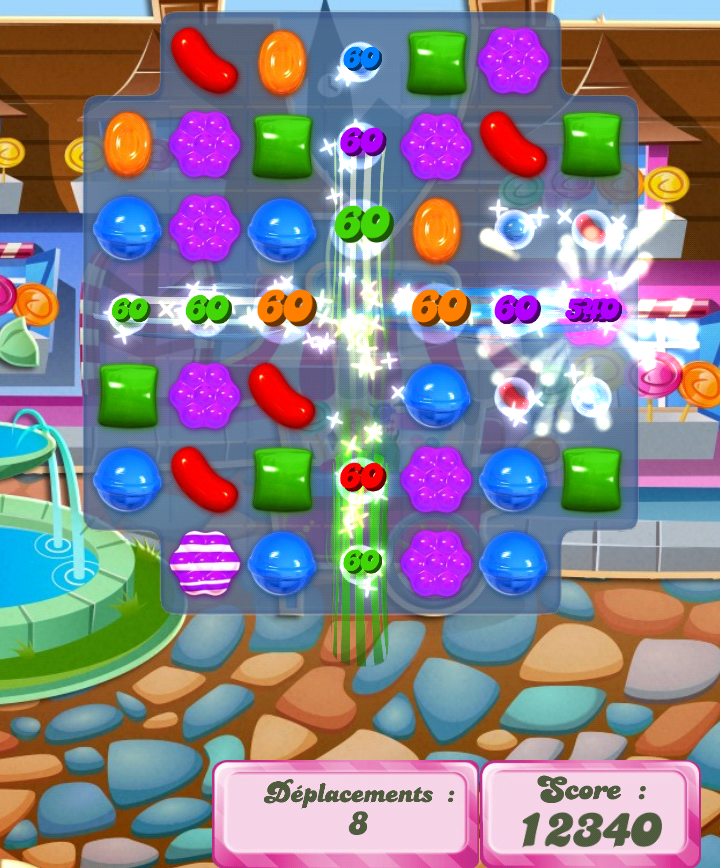
\includegraphics[width=\textwidth]{imgs/candyIntro.png}
				}{
					\begin{itemize}
						\item Développeur : King
						\item Sortie : 2012
						\item Puzzle
					\end{itemize}
				}
			\end{block}
		\end{column}
		\begin{column}{0.5\textwidth}
			\begin{block}{Centipede}
				\alt<2>{
					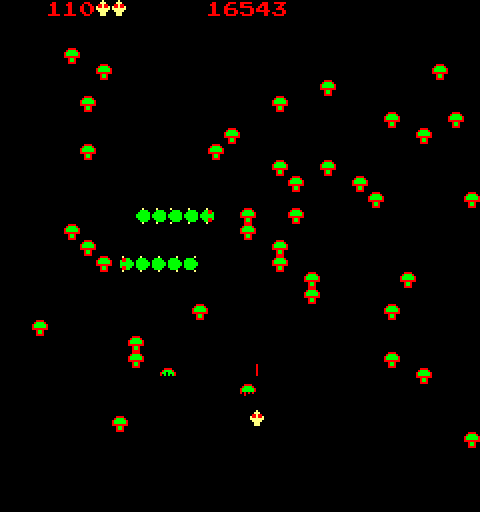
\includegraphics[width=\textwidth]{imgs/centipedeIntro.png}
				}{
					\begin{itemize}
						\item Développeur : Atari Inc.
						\item Sortie : 1981
						\item Shoot 'em up (arcade)
					\end{itemize}
				}
			\end{block}
		\end{column}
	\end{columns}
\end{frame}

\section{Jeu 1 : Candy Crush}
\subsection{État du jeu}
\begin{frame}{État du jeu}
	{\texttt{*} signifie constant}
	\begin{typeag}{Niveau}
		\variable{numeroNiveau}{entier}\\
		\variable{deplacementMax}{entier}\\
		\variable{deplacementUtilises}{entier}\\
		\variable{grille}{entier [tailleX][tailleY]}\\
		\variable{grilleDeDestruction}{boolean [tailleX][tailleY]}
	\end{typeag}
	~\\
	\begin{typeag}{Position}
		\variable{x}{entier}\\
		\variable{y}{entier}
	\end{typeag}
\end{frame}

\begin{frame}{État du jeu}
	{\texttt{*} signifie constant}
	\begin{typeag}{Case}
		\variable{caseADeplacer}{Position}\\
		\variable{caseCible}{Position}\\
		\variable{caseTemporaire}{entier}\\
		\variable{nbCasesAlignes}{entier}
	\end{typeag}
	~\\
	\begin{typeag}{Score}
		\variable{cible}{entier}\\
		\variable{actuel}{entier}
	\end{typeag}
\end{frame}

\subsection{Configuration initiale du jeu}
\begin{frame}{Configuration initiale du jeu}
	\begin{itemize}
		\item
			Décor: grille modulable selon le niveau
		\item
			Bonbons : 5 couleurs différentes
		\item
			Nombre de coups limité
		\item
			Jauge de points en fonction du score (0 au départ)
		\item
			Objectif à réaliser pour gagner
		\item 
			Viabilité : pas de combinaisons directes au départ
	\end{itemize}
\end{frame}

\subsection{Évolution de l'état du jeu}

\begin{frame}{Deplacement - vérification}
	\begin{columns}
		\begin{column}{0.49\textwidth}
			\begin{block}{Vérification}
				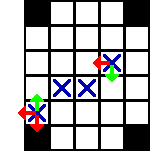
\includegraphics[width=\textwidth]{imgs/verifDepl}
			\end{block}
		\end{column}
		\begin{column}{0.49\textwidth}
			Vérifications :
			\begin{itemize}
				\item
					Déplacement dans la grille
				\item
					Déplacement sur case jouable
				\item
					Cases côtes à côtes
				\item
					Alignement de 3 ou plus
			\end{itemize}
		\end{column}
	\end{columns}
\end{frame}

\begin{frame}{Deplacement - détection et destruction}
	\begin{columns}
		\begin{column}{0.49\textwidth}
			\begin{block}{Détection}
				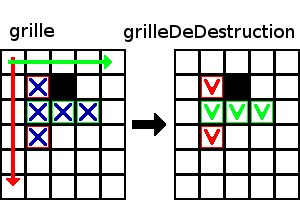
\includegraphics[width=\textwidth]{imgs/Detection}
			\end{block}
		\end{column}
		\begin{column}{0.49\textwidth}
			\begin{block}{Destruction}
				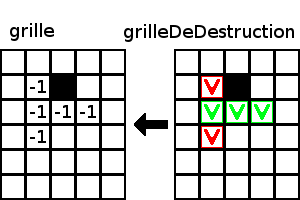
\includegraphics[width=\textwidth]{imgs/Destruction}
			\end{block}
		\end{column}
	\end{columns}
\end{frame}

\begin{frame}{Deplacement - remplacement}
	\begin{columns}
		\begin{column}{0.49\textwidth}
			\begin{block}{Tri des -1}
				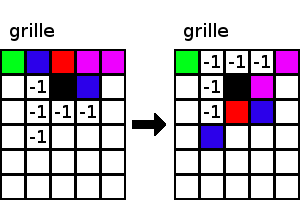
\includegraphics[width=\textwidth]{imgs/Remplacement1}
			\end{block}
		\end{column}
		\begin{column}{0.49\textwidth}
			\begin{block}{Tirage aléatoire des cases}
				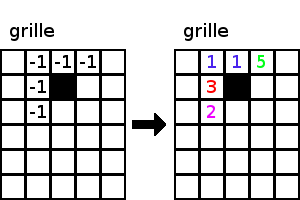
\includegraphics[width=\textwidth]{imgs/Remplacement2}
			\end{block}
		\end{column}
	\end{columns}
\end{frame}


\section{Jeu 2 : Centipede}
\subsection{État du jeu}
\begin{frame}{État du jeu}
	{\texttt{*} signifie constant} % Ça fait bizarre là où c'est mais ça gêne pas
	\begin{columns}
		\begin{column}{0.5\textwidth}
			\begin{typeag}{Personnage}
				\variable{vies}{entier}\\
				\variable{positionX}{entier}\\
				\variable{positionY}{entier}\\
				\variable{vitesse}{entier*}
			\end{typeag}
			\begin{typeag}{Champignon}
				\variable{vie}{entier}\\
				\variable{estVeneneux}{booléen}\\
				\variable{positionX}{entier}\\
				\variable{positionY}{entier}

			\end{typeag}
			\begin{typeag}{Projectile}
					\variable{actif}{booléen}\\
					\variable{vitesse}{entier}\\
					\variable{positionX}{entier ou réel}\\
					\variable{positionY}{entier ou réel}
			\end{typeag}
		\end{column}
		\begin{column}{0.5\textwidth}
			\begin{typeag}{Zone de jeu}
				\variable{champis}{Champignon[nbMax]}\\
				\variable{tir}{Projectile}\\
				\variable{couleurs}{entier}\\
				\variable{score}{entier}\\
				\variable{niveau}{entier}
			\end{typeag}
			\begin{typeag}{Segment}
				\variable{etat}{entier}\\
				\variable{vitesse}{entier}\\
				\variable{direction}{entier}\\
				\variable{positionX}{entier}\\
				\variable{positionY}{entier}
			\end{typeag}
			\variable{centipede}{Segment[12]}
		\end{column}
	\end{columns}
\end{frame}

\subsection{Configuration initiale du jeu}
\begin{frame}{Configuration initiale du jeu}
	\begin{typeag}{Personnage}
		\variablei{vies}{\texttt{2}}\\
		\variablei{positionX}{\texttt{largeurEcran/2}}\\
		\variablei{positionY}{\texttt{hauteurEcran-hauteurPersonnage}}\\
		\variablei{vitesse}{1 pixel par frame}\\
	\end{typeag}
	\begin{typeag}{Zone de jeu}
		\variablei{champis}{rempli par des champignons dispersés}\\
		\variablei{tir}{projectile inactif}\\
		\variablei{couleurs}{\texttt{0}}\\
		\variablei{score}{\texttt{0}}\\
		\variablei{niveau}{\texttt{1}}
	\end{typeag}
	\variablei{centipede}{jardin.niveau têtes puis des segments}
\end{frame}

\subsection{Évolution de l'état du jeu}
\begin{frame}{Entrées du joueur}
	\begin{columns}
		\begin{column}{0.4\textwidth}
			\begin{block}{Déplacement}
				Restreint :
				
				\smallskip
				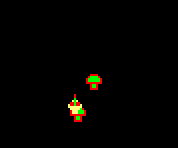
\includegraphics[width=\textwidth]{imgs/collisionChampignon.png}
			\end{block}
		\end{column}
		\begin{column}{0.4\textwidth}
			\begin{block}{Tir}
				Unique et libre :
				
				\smallskip
				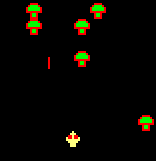
\includegraphics[width=\textwidth]{imgs/tirEtDeplacement.png}
			\end{block}
		\end{column}
	\end{columns}
\end{frame}
\begin{frame}{Évolution des éléments}
	\begin{columns}
		\begin{column}{0.3\textwidth}
			\begin{block}{Mort du joueur}
				Instantanée pour tout ennemi :
				
				\smallskip
				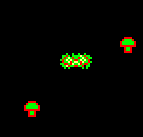
\includegraphics[width=\textwidth]{imgs/mortNain.png}
			\end{block}
		\end{column}
		\begin{column}{0.3\textwidth}
			\begin{block}{Tir/Ennemi}
				Destruction instantanée :
				
				\smallskip
				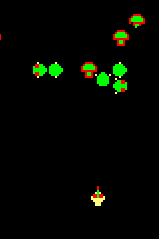
\includegraphics[width=\textwidth]{imgs/destructionSegment.png}
			\end{block}
		\end{column}
		\begin{column}{0.3\textwidth}
			\begin{block}{Champignons}
				Destructibles mais gênants pour le joueur et le centipède :
				
				\smallskip
				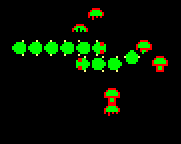
\includegraphics[width=\textwidth]{imgs/champignonsEtCentipede.png}
			\end{block}
		\end{column}
	\end{columns}
\end{frame}


\section{Conclusion}
\begin{frame}{Conclusion et remarques}
	\begin{block}{Remerciements}
		Merci de nous avoir écoutés
	\end{block}
	\begin{block}{Copyright}
		Nous avons pris les captures d'écrans à partir de versions en ligne de Centipede et à partir de Candy Crush Saga sur Android.

Les copyrights vont à leurs éditeurs respectifs.
	\end{block}
\end{frame}

\end{document}
